% THIS IS AN EXAMPLE DOCUMENT FOR VLDB 2012
% based on ACM SIGPROC-SP.TEX VERSION 2.7
% Modified by  Gerald Weber <gerald@cs.auckland.ac.nz>
% Removed the requirement to include *bbl file in here. (AhmetSacan, Sep2012)
% Fixed the equation on page 3 to prevent line overflow. (AhmetSacan, Sep2012)

\documentclass{vldb}
\usepackage{graphicx}
\usepackage{balance}  % for  \balance command ON LAST PAGE  (only there!)
\usepackage{cleveref}
\usepackage{times}

\newcommand\system{\textsc{SourceSight}}
\newtheorem{definition}{Definition}


\begin{document}

% ****************** TITLE ****************************************

\title{{\LARGE \system}: Enabling Effective Source Selection}

\numberofauthors{3} 

\author{
% 1st. author
\alignauthor
Theodoros Rekatsinas\\
       \affaddr{University of Maryland}\\
       \email{thodrek@cs.umd.edu}
% 2nd. author
\alignauthor
Amol Deshpande\\
       \affaddr{University of Maryland}\\
       \email{amol@cs.umd.edu}
% 3rd. author
\alignauthor 
Xin Luna Dong\\
       \affaddr{Google Inc.}\\
       \email{lunadong@google.com}
\and  % use '\and' if you need 'another row' of author names
% 4th. author
\alignauthor 
Lise Getoor\\
       \affaddr{UC Santa Cruz}\\
       \email{getoor@soe.ucsc.edu}
% 5th. author
\alignauthor Divesh Srivastava\\
       \affaddr{AT\& T Labs-Research}\\
       \email{divesh@research.att.com}
}

\maketitle

\begin{abstract}
Recently there has been a rapid increase in the number of data sources and publicly accessible data services, such as cloud-based data markets and data portals, that facilitate the collection, publishing and trading of data. Data sources typically exhibit large heterogeneity in the type and quality of data they provide. Unfortunately, when the number of data sources is large, users have a limited capability of reasoning about the actual usefulness of sources and the trade-offs between the benefits and costs of acquiring and integrating sources. In this demonstration we present \system, a framework that facilitates the exploration and selection of sources for integration. \system~is based on the intuition that different sets of data sources are optimal to integrate for different integration tasks. The main focus of \system~is to allow users to discover and explore valuable sets of sources for diverse integration tasks over large numbers of heterogeneous data sources.
\end{abstract}


\section{Introduction}
Data integration remains among the most cost-intensive tasks in data management, either because of the considerable computation and human-curation costs involved in the process~\cite{kruse2015estimating}, or the monetary cost involved in acquiring data~\cite{balazinska:vldb11}. Given the high number of available data sources and the aforementioned costs, it is challenging for a user to identify the sources that are truly beneficial to her application. This gives rise to the natural question of how can one discover {\em the most beneficial sources} for integration, i.e., sources that maximize the user's benefit at the minimum cost. 

Several approaches have been proposed to help users reason about the value of integrating multiple data sources. The proposed approaches can be divided into two main categories: (i) {\em effort-oriented} techniques that focus on characterizing solely the cost of integration, and (ii) {\em benefit-oriented} techniques that reason about the benefit of integration. Techniques from the first category estimate the cost of integration via reasoning about the effort required to perform schema-matching, data-cleaning and data-transformation when integrating multiple sources~\cite{kruse2015estimating, smith:2009}. While valuable at estimating the overall cost of integration, these techniques do not reason about the actual benefits of integrating multiple sources. On the other hand, benefit-oriented techniques put more emphasis on characterizing the benefit of integrating a new source based on its marginal gain~\cite{dong:vldb13,rekatsinas:2014}. Nevertheless, both approaches usually assume that users have already identified all the sources relevant to their application and do not allow users to explore and identify which sources are the most beneficial for their desired {\em integration task}. Moreover, they do not support diverse integration tasks across multiple users.

To understand these limitations, consider the scenario of biologists that want to combine diverse sources of information from functional genomics experiments to make large-scale predictions for protein-to-protein interaction networks. Each prediction task is associated with an {\em integration task} that is characterized by the organism and the genes the biologist is targeting. Results of such experiments are usually collected in repositories such as ArrayExpress\footnote{http://www.ebi.ac.uk/arrayexpress/}. However, such repositories contain vast amounts of experimental data (e.g., ArrayExpress has results from 56,369 different experiments) and while users can provide a description of their integration task (i.e., a description of the genes they are interested) they might not know all the experiments that are relevant to their task. Therefore it is of great importance to allow users to discover and select sources based purely based on their integration task description. Moreover, such repositories are not limited to specific experiments but are designed to support diverse tasks posed by multiple users. For example, one group of users might be interested in human protein-to-protein interaction networks ~\cite{humanpp} and others in yeast protein-to-protein networks~\cite{yeastpp}.

Recently, we introduced our vision for a {\em data source management system}~\cite{rekatsinas:2015} that enables users to discover the most valuable sources for their applications and described a preliminary system design that can support diverse integration scenarios and can help users truly understand the quality and cost trade-offs between different integration options. In this demonstration proposal, we present \system, a fully functional prototype of such a data source management system. We also discuss extensions to our initial design that allow user to evaluate the effectiveness of the system (\Cref{sec:extensions}). The core of the system is built around the paradigm of {\em source selection}~\cite{dong:vldb13} that allows one to reason about the trade-offs between the gain and cost of integration. The gain of integration can be quantified using a variety of data quality metrics, such as coverage, accuracy, timeliness and bias. The cost of integration is quantified using a model similar to that of Dong et al.~\cite{dong:vldb13}, however, other cost models such as the one introduced by Kruse et al.~\cite{kruse2015estimating} can be seamlessly incorporated in our system. \system~offers a number of unique features:

\vspace{2pt}\noindent (1) Users can describe the domain of their desired integration task using a keyword-based interface. Moreover, the system allows them to explore similar or related domains refining the description of their desired task. Simultaneously users have the opportunity to explore sources that are highly relevant to their desired task.

\vspace{2pt}\noindent (2) Given a desired integration task, users can perform source selection using a variety of quality metrics. \system~casts source selection as a multi-variate optimization problem to help users understand the actual trade-offs between different quality metrics and proposes multiple sets of sources to be used when different weights are assigned to different quality metrics. 

\vspace{2pt}\noindent (3) Finally, the system allows users to edit the recommended solutions by adding or deleting sources. Users can also perform a qualitative comparison between different sets of sources. This is crucial for evaluating the solutions recommended by \system~and aids the users to understand why the particular set of sources was proposed by the system.

In the following sections, we describe the organization of the demonstration. First, we review what it means for a user to discover valuable sources for a specified integration task (\Cref{sec:sources}). Then we present an overview of the architecture of \system~and describe its core functionalities and discuss how they enable effective source selection for diverse integration tasks (\Cref{sec:design}). Finally, we provide an outline of the \system~use cases that VLDB attendees will experience during the demo (\Cref{sec:details}).

\vspace{2pt}\noindent\textbf{Related work.}

\section{Discovering Valuable Sources \\ with {\Large \system}}
Consider a scenario where users interact with a repository that stores the raw data from multiple sources and want to identify sources relevant to a desired integration task. In \Cref{sec:intro}, we presented an example of biologists interacting with ArrayExpress but other use cases include scientists that share their experimental results and collaborate on large-scale datasets via a repository such as DataHub~\cite{datahub}, or business analysts that want to acquire data from a marketplace~\cite{balazinska:vldb11}, such as Datasift\footnote{http://datasift.com/} or journalists that want to write an overview article and want to compile information from multiple news sources stored in a single repository such as EventRegistry\footnote{http://eventregistry.org/}. 

Sources in such repositories usually exhibit large heterogeneity with respect to the data they provide as they may provide stale or erroneous data~\cite{Dong_vldb:2009, li:2012}, they may contain duplicate data~\cite{bronzi:2013, li:2012} at different prices, and may exhibit schema or data instance heterogeneity (e.g., provide synonym mentions to the same real-world entities). Moreover, as discussed previously, we assume that users do not know all sources that are relevant to their integration task.

For example, consider a journalist that wants to write an overview article about the socio-economic situation in ``Greece'' but has a limited budget (e.g., wants to review a limited number of news sources due to time constraints). The fist step for the journalist is to explore which sources are relevant to her task but also which specific contexts might be related to the initial description. Then she wants to 

\section{Discovering Valuable Sources \\ with {\Large \system}}
\label{sec:sources}
We consider a scenario where users interact with a system that stores and manages data sources under a single repository and want to identify sources relevant to a desired integration task. Examples of such repositories may correspond to data marketplaces~\cite{balazinska:vldb11}, data portals, such as Datasift\footnote{http://datasift.com/}, or online platforms for organizing, managing and sharing datasets~\cite{datahub}. 

Sources can exhibit large heterogeneity with respect to the data they provide. We assume that each entry in a source is associated with a set of {\em context literals} and all context literals come from a {\em literal dictionary} $V$. This dictionary $V$ may follow a structured form, e.g., be a knowledge-base, describing how different literals are related to each other. For example, if the source entries correspond to structured entries these literals may correspond to the values for a subset of attributes of each entry (e.g., the location value and business type value for business listings). If the source entry corresponds to unstructured free-text data, these literals may correspond to {\em real-world entities} or {\em concepts} from a knowledge-base. The aforementioned assumptions allow one to reason about the domain covered by each source by analyzing the union of context-literal sets associated with the entries of the source. 

We also consider that a user integration task $I = (I_d, I_c)$ is fully specified by a description that corresponds to a context-literal set $I_d$ defining the {\em domain} of the task and potentially a set of integration cost or effort constraints $I_c$. Discovering the most valuable sources for task $I$ requires performing the following operations: (i) identifying the relevant sources for task $I$, (ii) discovering sets of sources that if integrated together will maximize the {\em benefit} of integration under the constraints $I_c$. 

Relevant sources to task $I$ are all data sources that provide entries whose context-literal set is a subset of $I_d$. Not of all these sources may be beneficial for task $I$ as sources may provide stale or erroneous data~\cite{Dong_vldb:2009, li:2012}, or may provide duplicate data~\cite{bronzi:2013, li:2012} at different prices. In our recent work~\cite{dong:vldb13,rekatsinas:2014, rekatsinas:2015} we showed how
, given a fixed data domain, the benefit of integration can be quantified using rigorous data quality metrics, such as {\em coverage}, {\em accuracy}, {\em timeliness} or {\em bias}, and introduced the paradigm of {\em source selection} to detect the most beneficial sources for integration by reasoning about the benefits and costs of acquiring and integrating data. 

Consider an integration task $I = (I_d, I_c)$ and let $S$ denote the set of all sources relevant to $I$. Assume an oracle $\mathbf{G_q}(\cdot)$ that takes as input a set of sources $\bar{S}$ and a set of context-literals $I_d$ and returns the a vector containing the gain of integrating sources $\bar{S}$ with respect to the different quality metrics $q$. Moreover, let $C(\cdot)$ be an oracle that takes as input a set of sources $\bar{S}$ and returns the total integration cost. The result of source selection corresponds to a sets of sources $S_I$ such that $S_I = \arg\max_{\bar{S} \subseteq S}\mathbf{G_q}(\bar{S},I_d) - C(\bar{S})$.

%\section{Discovering Valuable Sources}
%  We consider a scenario where users interact with a system that stores and manages data sources under a single repository and want to identify sources relevant to a desired integration task. Examples of such repositories may correspond to data marketplaces~\cite{balazinska:vldb11}, data portals, such as Datasift\footnote{http://datasift.com/}, or online platforms for organizing, managing and sharing datasets~\cite{datahub}. In this section we describe the main functionalities that such systems needs to support to allow users to discover sources that are the most beneficial for a desired integration task. 
%
%\subsection{Reasoning about The Content of Sources}
%Sources may exhibit large heterogeneity with respect to the data they provide. To reason about the content of sources we assume that each entry in a source is associated with a set of {\em context literals}. We assume that all context literals come from a {\em literal dictionary} $V$. Moreover, we assume that the dictionary $V$ may follow a structured form, e.g., be a knowledge-base, describing how different literals are related to each other. For example, if the source entries correspond to structured entries these literals may correspond to the values for a subset of attributes of each entry (e.g., the location value and business type value for business listings). If the source entry corresponds to unstructured free-text data, these literals may correspond to {\em real-world entities} or {\em concepts} from a knowledge-base. Following this assumption, a data-source repository can reason about the domain covered by each source by analyzing the union of context-literal sets associated with the entries of the source. 
%
%\subsection{Describing the Integration Task}
%Typically a user would start by proving a description of her desired integration task as well as any requirements (e.g., requirements on the total effort of integration) characterizing the task. We assume that users can describe a desired integration task using a set of context literals that belong in the dictionary $V$. Integration-task requirements can correspond to constraints on the total number of sources used for integration or explicit budget constraints on the cost or total effort of integration.
%
%Given an integration task $I$ described by a  context-literal set $I_c$, the system can {\em recommend}.
%
%
%\subsection{Multi-variate Source Selection}
%Given a finalized integration task $I$ associated with a context-literal set $I_c$ the system automatically finds subsets of sources that, if integrated together, maximize the benefit of integration under the budget requirements of the user. If available, the system identifies multiple solutions that correspond to different trade-offs among different quality metrics.
%
%The discovered solutions are presented to the user together with a concise description of their quality characteristics as well as a description of the data sources included in each of thi think em. 
%
%\subsection{Providing Explanations}
%
%analyze the content of sources, identify the domains that sources cover and materialize quality profiles. 
%
%Different quality metrics available 
%
%Users provide a query that specifies a domain
%
%Oracle provides the quality profiles of sources for the specified domain
%
%Perform source selection

\section{{\Large \system} Design}
\label{sec:design}
In a recent paper~\cite{rekatsinas:2015}, we put forward our vision about the functionalities that data source management systems should support to facilitate effective source selection and the architecture they should follow. 
\system~is a realization of our vision for such a system. Next, we describe \system's architecture, the different functionalities it supports and extensions of the preliminary design implemented in \system.%

\subsection{Architecture overview}
\system-is built as a layer on top of a data source repository, that stores the raw data of data sources. The system consists of three components: a frontend, a source analysis engine and a query engine. The frontend is a ``thin client'' that is used to specify integration tasks and display visualizations that aid users to select the desired sources for integration. The source analysis engine processes the raw data from the available data sources to identify the content of sources, and also evaluates their quality with respect to different quality metrics such as the ones described in the previous section. Finally, the query engine takes as input user-specified requirements and performs the necessary computation to serve those. The architecture of \system~is presented in \Cref{fig:architecture}. 

\begin{figure}[h]
    \centering
    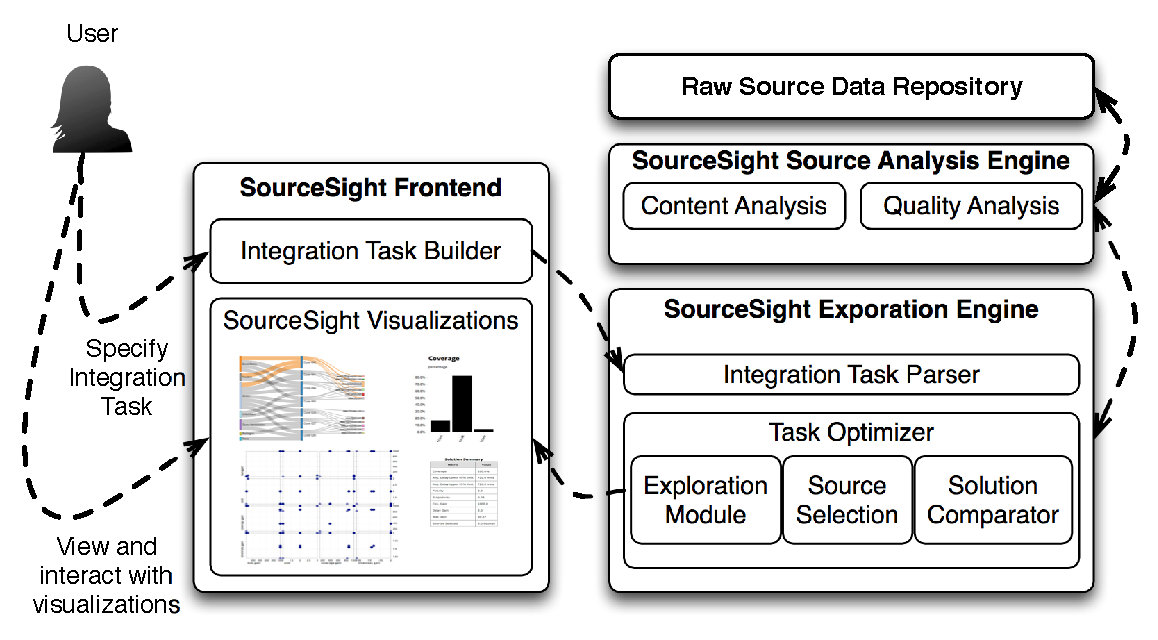
\includegraphics[width=0.48\textwidth]{fig/srcsightOver}
    \caption{\system~architecture.}
    \label{fig:architecture}
\end{figure}

The basic operations of \system~can be divided into an {\em offline} phase and an {\em online} phase. At the offline phase, the source analysis module constructs an index describing both the content and the quality of each source with respect to multiple quality metrics. This index is used during the online phase when a user interacts with the system to serve the user requests. We discuss the indexing technique in more detail in \Cref{sec:reasoning}. At the online phase users interact with \system~via its frontend module and user requests are served by the query engine. Users can specify a desired integration task by providing a free-text description of the context literals that describe the task. Once a description is provided users can choose among three main functionalities with respect to the specified integration task. They can (i) choose to explore which context literals and sources are highly relevant to the specified task, (ii) choose to perform source selection, or (iii) choose to perform a qualitative comparison between different sets of sources constructed either manually or automatically via source selection. The first functionality allows a user to refine her integration task specification by exploring related contexts. It also allows users to obtain an overview of the quality of individual sources (see \Cref{sec:integtask}). The second functionality returns multiple recommended source selection solutions with respect to a variety of quality metrics (see \Cref{sec:sourcesel}). Finally, \system~allows users to compare and contrast different sets of sources to further understand the benefits of choosing a specific set and understand why the particular set was recommended by source selection (see \Cref{sec:extensions}). We now discuss the different components in detail.

\subsection{Reasoning about the content of sources}
\label{sec:reasoning}
As discussed in \Cref{sec:sources}, we assume that each source entry is associated with a set of context literals coming from a literal dictionary $V$. Moreover, we assume the existence of a {\em knowledge base} (or ontology) describing relations amongst the literals in $V$.  To reason about the content of different sources and their data quality we recently proposed augmenting such a knowledge base with a {\em correspondence graph}~\cite{rekatsinas:2015}. 
\begin{figure}
	\begin{center}
	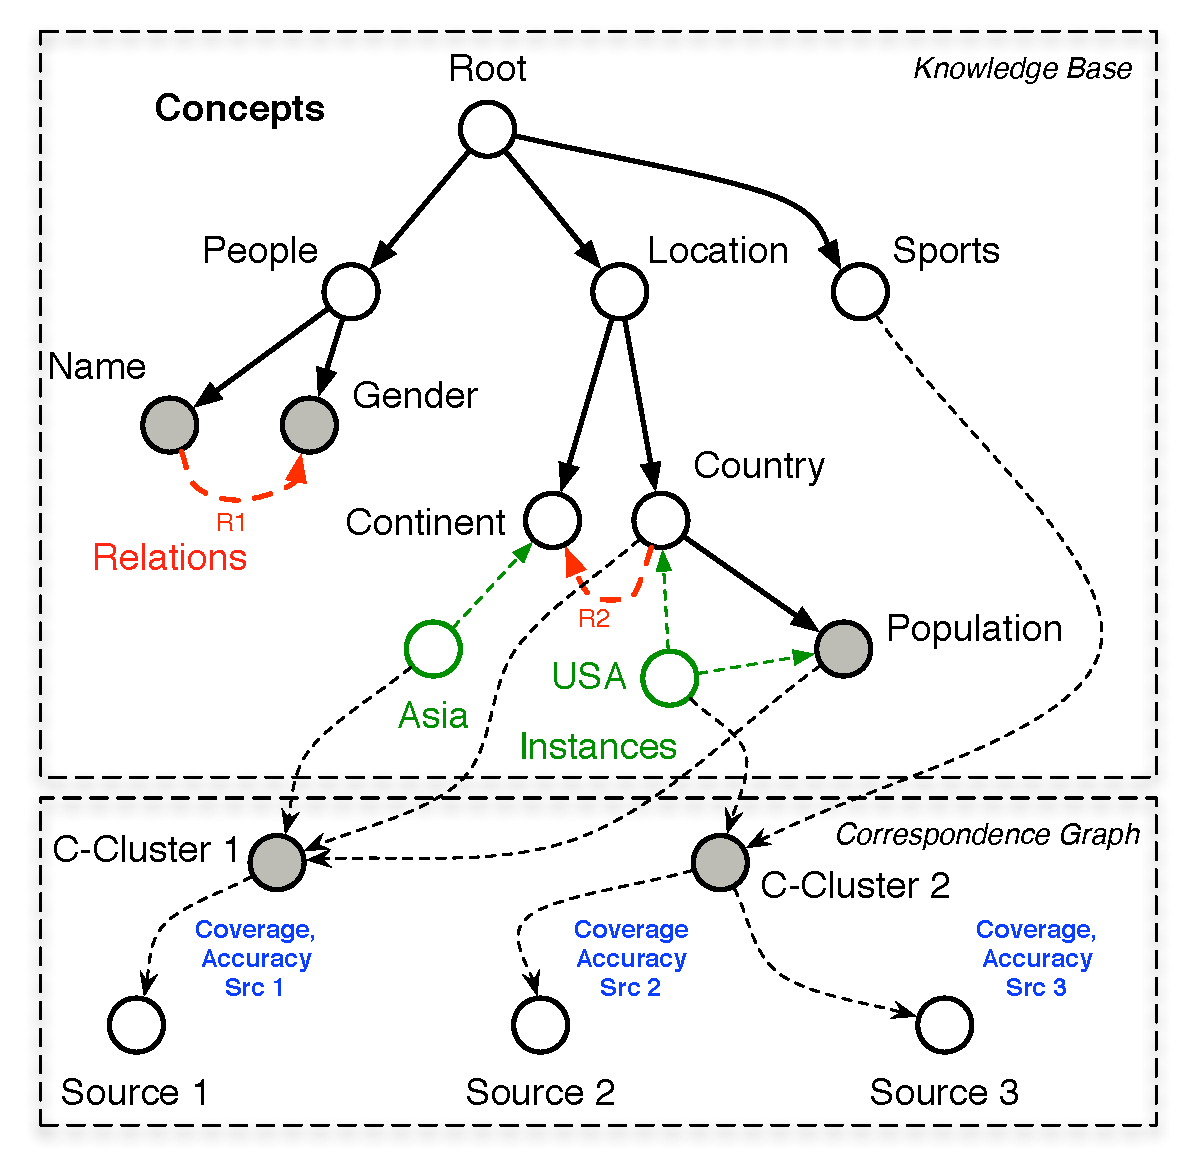
\includegraphics[clip,scale=0.25]{fig/kgcg}
	\caption{An example of a knowledge base and a correspondence graph with two c-cluster nodes corresponding to the population of countries in Asia and sports in the USA.}
	\label{fig:kgcg}
	\vspace{-20pt}
	\end{center}
\end{figure}
Specifically, the nodes in the correspondence graph are either data sources (referred to as {\em source nodes}) or c-clusters of concepts and/or entities as dictated by the available sources (called {\em c-cluster nodes}). The edges in the correspondence graph connect each source node with c-cluster nodes and c-cluster nodes with the corresponding concepts and entities in the knowledge base.  Each edge from a source to a c-cluster node is annotated with a quality profile of that source for that specific c-cluster, and each c-cluster node is associated with local information about the dependencies of the data sources that are connected to it. An example of a knowledge base and a correspondence graph is shown in \Cref{fig:kgcg}. There are two c-cluster nodes, one corresponding to the population of countries in Asia and one to sports in the USA. 

The correspondence graph serves as a content and quality index for the available sources. To construct it we first learn the latent c-cluster nodes and then compute the quality profiles and data source dependencies for each c-cluster node. To discover the literals associated with each source entry we use Thomson Reuter's Open Calais\footnote{http://www.opencalais.com/}, an API for semantic annotations with respect to multiple knowledge bases including DBpedia, Freebase and others. To construct the c-cluster nodes we adopt a frequent pattern mining approach based on the FP-growth algorithm~\cite{Han:2000}.  After discovering the c-cluster nodes, we compute the quality of each source with respect to each c-cluster node it is connected to. For the latter, we collectively analyze the content of all sources connected to a c-cluster node following an approach similar to Rekatsinas et al.~\cite{rekatsinas:2014} where samples from all the sources are integrated into a single dataset forming the content of the c-cluster and then each individual sample is compared with the integrated data to compute the source quality. 

\subsection{Specifying and Refining an Integration Task}
\label{sec:integtask}
\system~allows users to specify their desired integration task via a keyword search interface where keywords are matched against context literals in the knowledge base and correspondence graph. The system offers users with the functionality of exploring literals and sources that are related to their keyword search enabling them to explore similar integration tasks or refine their initial task. \Cref{fig:exploration} shows an example exploration scenario and the corresponding visualizations offered by \system. Consider a user searching data sources that mention things about ``Greece''.  \system~returns a set of relevant literals to the search of the user as well as the most relevant sources with respect to coverage for the specified keyword search. As shown some of the literals related to ``Greece" correspond to the concepts of ``Business and Finance'', ``Environment''', ``Sports'', etc. Given these literals the user may choose to further specialize her search and specify her task as ``Greece, Business, Finance''. As shown in \Cref{fig:exploration}, \system~will update the corresponding visualization with a new set of related literals (here ``Athens'', ``EUR'', ``Bank of Greece'', etc.) and provide the user with an updated set of relevant sources. The user can select any of the recommended sources to view a summary of the literals that the source covers as well as a quality summary of the source for the corresponding keyword search.
\begin{figure}
	\begin{center}
	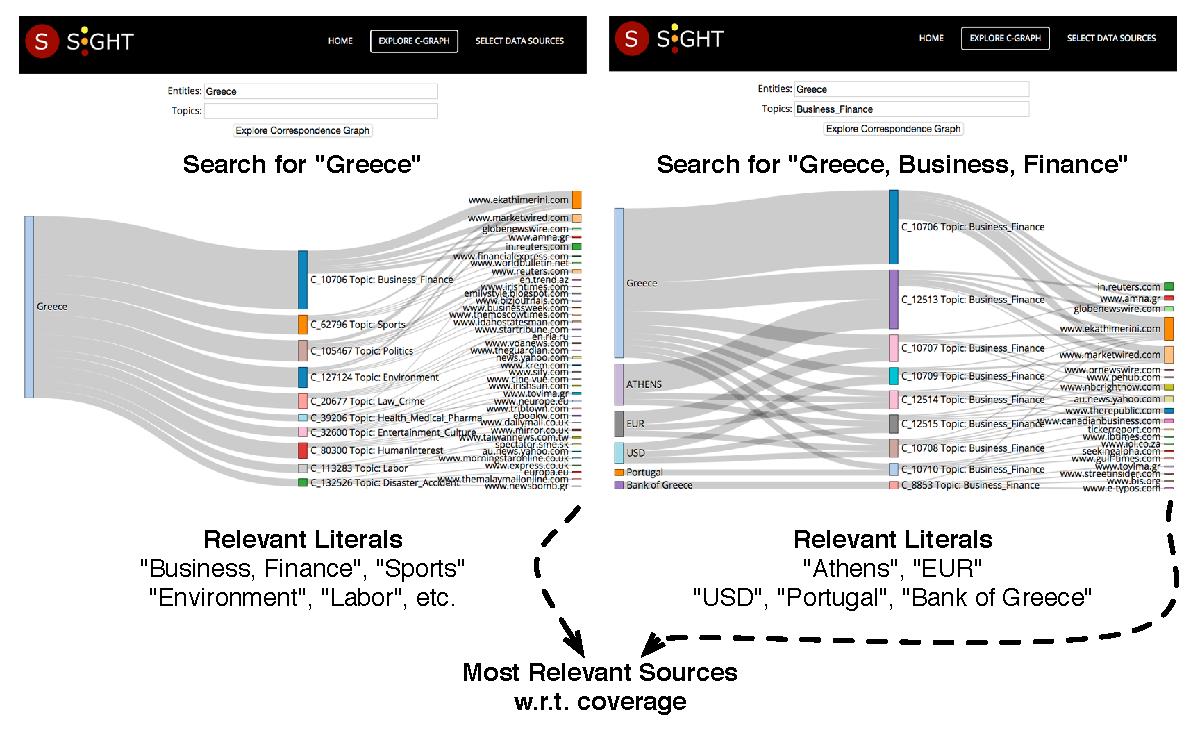
\includegraphics[trim=0 0 0 60, clip,width=0.48\textwidth]{fig/exploreCor}
	\caption{An example of a knowledge base and a correspondence graph with two c-cluster nodes corresponding to the population of countries in Asia and sports in the USA.}
	\label{fig:exploration}
	\end{center}
\end{figure}

\subsection{Multi-variate Source Selection}
\label{sec:sourcesel}
Once a user has identified the context literal description that fully specifies her integration task (via keyword search), she can perform source selection with respect to that set of literals. As mentioned in \Cref{sec:sources}, source selection considers multiple quality metrics to quantify the benefit of integration. \system~casts source selection as a multi-objective optimization problem and the query engine finds the set of {\em Pareto optimal} solutions corresponding to the source selection problem at hand. 

\begin{figure}
	\begin{center}
	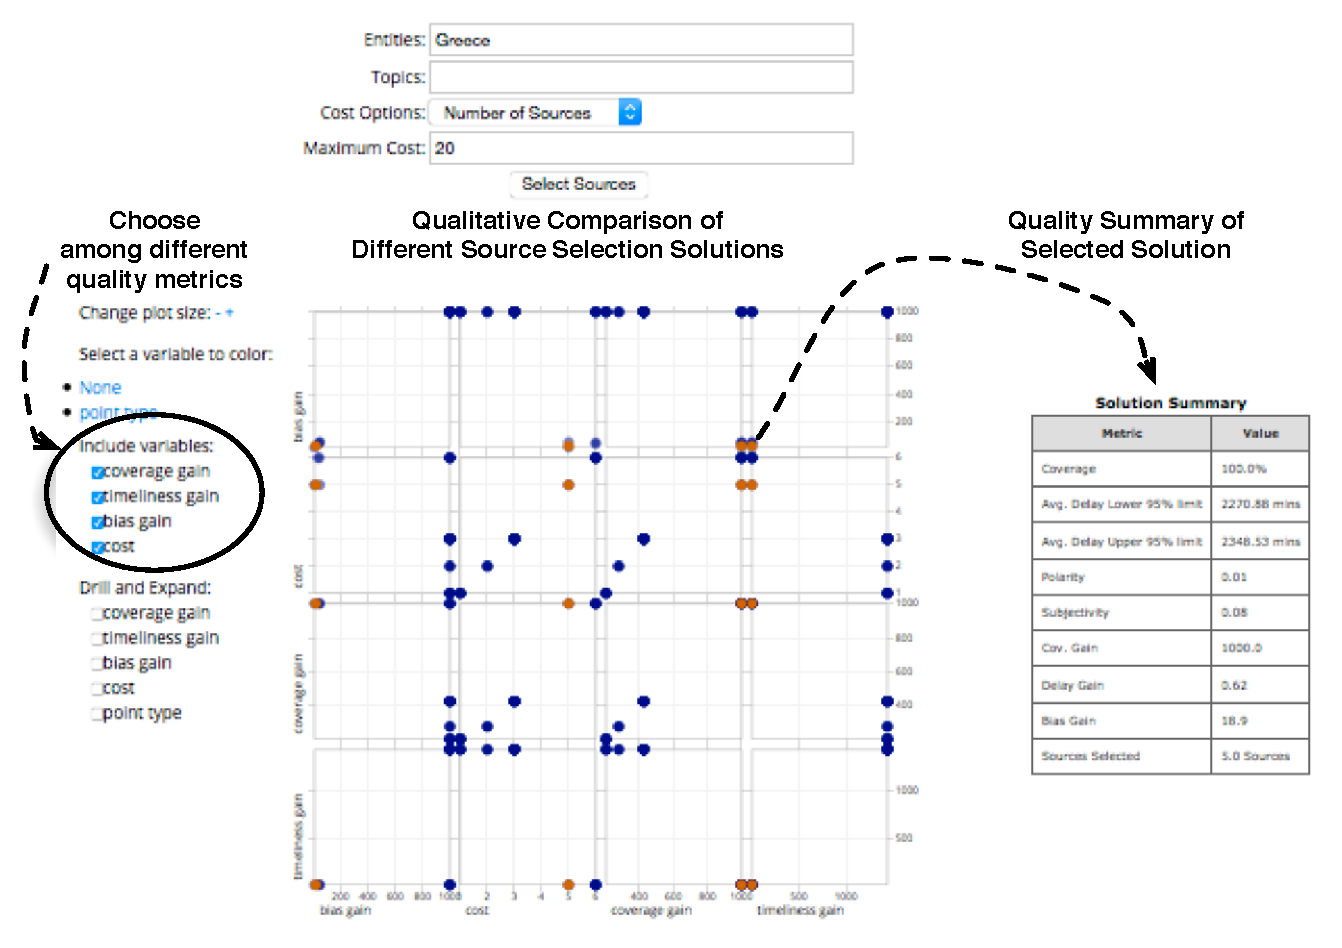
\includegraphics[trim=0 0 0 85, clip,width=0.48\textwidth]{fig/ssResults}
	\caption{\system's interface for exploring different source selection solutions.}
	\label{fig:ssresults}
	\end{center}
\end{figure}

Discovering all the solutions on the Pareto front is expensive as one needs to reason about all the potential trade-offs amongst the available quality metrics. To address this issue we use a {\em sampling} strategy to recover solutions that correspond to different quality trade-offs. More precisely, let $Q$ is the set of quality metrics under consideration and $G_q(\cdot)$ be an oracle computing the gain of integration with respect to quality metric $q \in Q$ for any set of sources. We compute the total gain of integration as a weighted linear combination of the individual gain for each quality metric, i.e., $G(\cdot) = \sum_{q \in Q} w_q \cdot G_q(\cdot)$. Given this definition of the total gain of integration, we sample different combinations for the weights $w_q$ and solve source selection for each of those. Finally we identify the Pareto optimal solutions amongst of sampled solutions. 

All the sampled solutions are presented to the user in a way that is easy for her to compare the quality of each solution. The corresponding interface is shown in \Cref{fig:ssresults}. Users can select a particular solution and view a concise summary of the gain and cost of integration achieved by it. Moreover,  users have the flexibility to drill and expand only on a subset of the available quality metrics. This allows them to fully understand specific trade-off across different solutions. Finally, can view a more detailed description of a proposed source selection solution including information such as the sources included in the result and their individual contributions to the quality of the final integration result. 

\subsection{Comparing and Contrasting Sets of Sources}
\label{sec:extensions}
Both functionalities presented above were alluded to our visionary paper on data source management systems~\cite{rekatsinas:2015}. Next, we discuss an analytical functionality in \system~that enables users to understand why a particular set of sources was recommended to them and evaluate the performance of the system.

\system~allows users to perform a qualitative comparison between two sets of sources with respect to the same integration task. The corresponding interface is shown in \Cref{fig:comparison}. In particular, users will be able to examine how the two sets of sources compare against each other with respect to individual quality metrics, as well as the total integration gain and cost. The aforementioned sets of source can either be selected directly from the solutions of source selection or can be manually constructed by the user. \system~offers two ways of manually specifying sets of sources: (i) users can start from a running source selection solution and add new sources or remove sources already included in the set, or (ii) users can manually select different sources and construct their own set. The former allows them to examine the neighborhood of the corresponding solution but also serves as a mechanism of convincing the user of the benefit achieved by the output of source selection. To enable the latter, \system~provides users with the top-k most relevant sources with respect to their integration task. As users select sources the ranking is revised to contain sources that are more beneficial given the current selection of the user. We point out that the rankings are computed with respect to the individual additional benefit of each source. 
\begin{figure}
	\begin{center}
	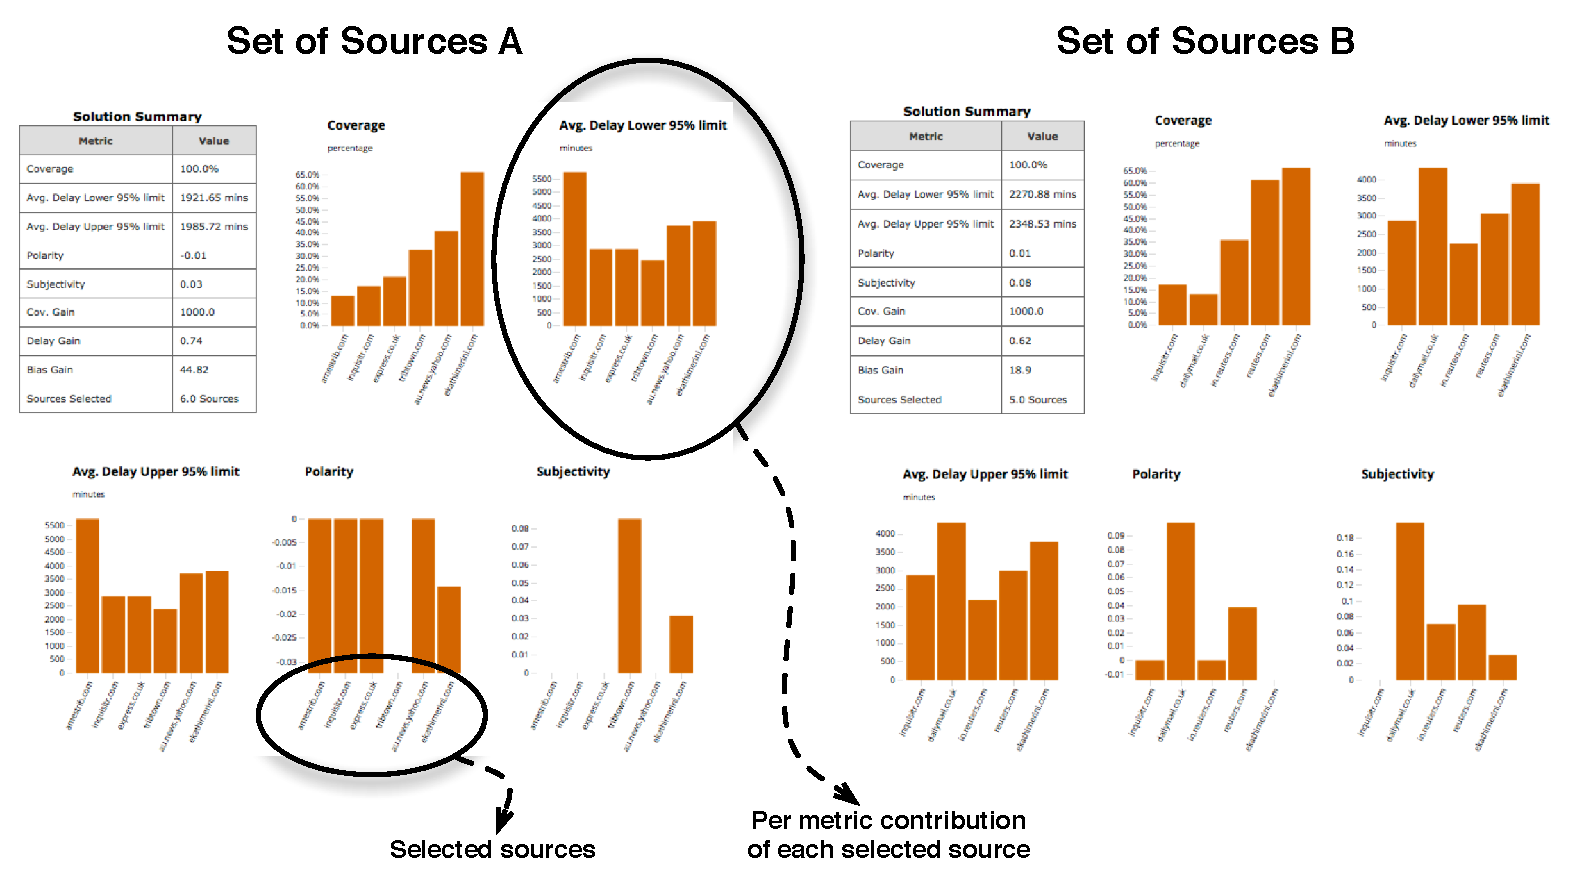
\includegraphics[trim=0 0 0 0, clip,width=0.48\textwidth]{fig/compSS}
	\caption{Comparing sets of sources.}
	\label{fig:comparison}
	\end{center}
\end{figure}

\section{Demo Details}
\label{sec:details}
We will demonstrate the functionality of \system~through hands-on experience with two large scale real-world datasets. The data will be stored on a remote server and users will interact with the system via a web interface. Our goals are two fold: (i) demonstrate the utility of \system~in exploring and selecting beneficial sources for integration and (ii) demonstrate the effectiveness of automatic source selection techniques for diverse scenarios. 

\vspace{2pt}\noindent\textbf{Datasets.} The first dataset we will use corresponds to event extractions collected from EventRegistry\footnote{http://eventregistry.org/}, a repository that monitors news media from all over the world and extracts geo-referenced records that correspond to different news articles. Data sources correspond to different news domains and quality metrics such as coverage, timeliness or position bias of the articles are inherently relevant. EventRegistry gets updated at fixed intervals  by ingesting feeds of newly extracted news articles. We believe that EventRegistry is the right fit to demonstrate the usefulness and practicality of \system~due to the large number of data sources available, the available updates over time, and the heterogeneity that the sources exhibit both with respect to their domain and their quality. We plan to use a recent snapshot retrieved from EventRegistry containing at least six months of news article data. 

The second dataset we will use corresponds to a Twitter snapshot. Here, individual Twitter users can be viewed as sources. Twitter gives its users an unprecedented ability to deliver news as developments unfold and has been adopted by many researchers as the means of predicting occurrences of events in the future. Hence, we believe that analyzing collections of tweets via \system~to identify sets of ``influential'' or ``trustworthy'' twitter users by employing source selection techniques would be of great interest to the VLDB participants.

\vspace{2pt}\noindent\textbf{Demonstrating Utility.} Attendees will be able to describe ad-hoc or pre-formulated integration tasks in \system. Then they will have the opportunity to evaluate the source exploration and source selection functionalities offered by \system~(described in \Cref{sec:integtask} and \Cref{sec:sourcesel}) with respect to these tasks. Our goal is for users to understand the trade-offs between different quality metrics of sources in both datasets we have described above and understand how \system~can guide them to select the most suitable set of sources for their application needs.

\vspace{2pt}\noindent\textbf{Demonstrating Effectiveness.} For this part of the demo users will mainly interact with the third functionality of \system, i.e., comparing and contrasting sets of sources. Attendees will have the opportunity to compare sets of sources provided by source selection with manually created sets of sources and understand the quality differences across them. To facilitate manual selection of sources, we will provide users with ranking mechanisms that consider each source in isolation for each individual quality metric. Starting from the recommended ranked sources users will be able to form their own set of sources by adding or removing sources and compare it with sets generated by \system. 

Overall, the demo will allow users to: (i) understand the internal source indexing mechanism (i.e., the correspondence graph) of our prototype system, (ii) issue queries against it and (iii) explore the corresponding source selection solutions via a web-interface. Users will need to play the role of an analyst and use our system to discover the most valuable sources for their own analysis applications.

{\small 
\bibliographystyle{abbrv}
\bibliography{srcsight}}

\end{document}
